% Options for packages loaded elsewhere
\PassOptionsToPackage{unicode}{hyperref}
\PassOptionsToPackage{hyphens}{url}
%
\documentclass[
  letterpaper,
  ignorenonframetext,
  aspectratio=43,
  handout,
  12pt]{beamer}
\usepackage{pgfpages}
\setbeamertemplate{caption}[numbered]
\setbeamertemplate{caption label separator}{: }
\setbeamercolor{caption name}{fg=normal text.fg}
\beamertemplatenavigationsymbolsempty
% Prevent slide breaks in the middle of a paragraph
\widowpenalties 1 10000
\raggedbottom
\setbeamertemplate{part page}{
  \centering
  \begin{beamercolorbox}[sep=16pt,center]{part title}
    \usebeamerfont{part title}\insertpart\par
  \end{beamercolorbox}
}
\setbeamertemplate{section page}{
  \centering
  \begin{beamercolorbox}[sep=12pt,center]{part title}
    \usebeamerfont{section title}\insertsection\par
  \end{beamercolorbox}
}
\setbeamertemplate{subsection page}{
  \centering
  \begin{beamercolorbox}[sep=8pt,center]{part title}
    \usebeamerfont{subsection title}\insertsubsection\par
  \end{beamercolorbox}
}
\AtBeginPart{
  \frame{\partpage}
}
\AtBeginSection{
  \ifbibliography
  \else
    \frame{\sectionpage}
  \fi
}
\AtBeginSubsection{
  \frame{\subsectionpage}
}
\usepackage{amsmath,amssymb}
\usepackage{lmodern}
\usepackage{ifxetex,ifluatex}
\ifnum 0\ifxetex 1\fi\ifluatex 1\fi=0 % if pdftex
  \usepackage[T1]{fontenc}
  \usepackage[utf8]{inputenc}
  \usepackage{textcomp} % provide euro and other symbols
\else % if luatex or xetex
  \usepackage{unicode-math}
  \defaultfontfeatures{Scale=MatchLowercase}
  \defaultfontfeatures[\rmfamily]{Ligatures=TeX,Scale=1}
\fi
\usetheme[]{metropolis}
% Use upquote if available, for straight quotes in verbatim environments
\IfFileExists{upquote.sty}{\usepackage{upquote}}{}
\IfFileExists{microtype.sty}{% use microtype if available
  \usepackage[]{microtype}
  \UseMicrotypeSet[protrusion]{basicmath} % disable protrusion for tt fonts
}{}
\makeatletter
\@ifundefined{KOMAClassName}{% if non-KOMA class
  \IfFileExists{parskip.sty}{%
    \usepackage{parskip}
  }{% else
    \setlength{\parindent}{0pt}
    \setlength{\parskip}{6pt plus 2pt minus 1pt}}
}{% if KOMA class
  \KOMAoptions{parskip=half}}
\makeatother
\usepackage{xcolor}
\IfFileExists{xurl.sty}{\usepackage{xurl}}{} % add URL line breaks if available
\IfFileExists{bookmark.sty}{\usepackage{bookmark}}{\usepackage{hyperref}}
\hypersetup{
  hidelinks,
  pdfcreator={LaTeX via pandoc}}
\urlstyle{same} % disable monospaced font for URLs
\newif\ifbibliography
\usepackage{longtable,booktabs,array}
\usepackage{calc} % for calculating minipage widths
\usepackage{caption}
% Make caption package work with longtable
\makeatletter
\def\fnum@table{\tablename~\thetable}
\makeatother
\usepackage{graphicx}
\makeatletter
\def\maxwidth{\ifdim\Gin@nat@width>\linewidth\linewidth\else\Gin@nat@width\fi}
\def\maxheight{\ifdim\Gin@nat@height>\textheight\textheight\else\Gin@nat@height\fi}
\makeatother
% Scale images if necessary, so that they will not overflow the page
% margins by default, and it is still possible to overwrite the defaults
% using explicit options in \includegraphics[width, height, ...]{}
\setkeys{Gin}{width=\maxwidth,height=\maxheight,keepaspectratio}
% Set default figure placement to htbp
\makeatletter
\def\fps@figure{htbp}
\makeatother
\setlength{\emergencystretch}{3em} % prevent overfull lines
\providecommand{\tightlist}{%
  \setlength{\itemsep}{0pt}\setlength{\parskip}{0pt}}
\setcounter{secnumdepth}{-\maxdimen} % remove section numbering
\usepackage{pgfpages}
\pgfpagesuselayout{2 on 1}
\providecommand{\tightlist}{%
\setlength{\itemsep}{0pt}\setlength{\parskip}{0pt}}
\makeatletter
\makeatother
\let\Oldincludegraphics\includegraphics
\renewcommand{\includegraphics}[2][]{\Oldincludegraphics[width=\textwidth,height=0.7\textheight,keepaspectratio]{#2}}
\ifluatex
  \usepackage{selnolig}  % disable illegal ligatures
\fi

\author{}
\date{}

\begin{document}

\begin{frame}{AE 737: Mechanics of Damage Tolerance}
\protect\hypertarget{ae-737-mechanics-of-damage-tolerance}{}
Lecture 2 - Common Stress Intensity Factors

Dr.~Nicholas Smith

Wichita State University, Department of Aerospace Engineering

3 February, 2021
\end{frame}

\begin{frame}{schedule}
\protect\hypertarget{schedule}{}
\begin{itemize}
\tightlist
\item
  3 Feb - Common Stress Intensity Factors
\item
  8 Feb - Superposition, Compounding
\item
  10 Feb - Curved Boundaries, HW 1 Due
\item
  15 Feb - Plastic Zone
\end{itemize}
\end{frame}

\hypertarget{review}{%
\section{review}\label{review}}

\begin{frame}{fracture mechanics}
\protect\hypertarget{fracture-mechanics}{}
\begin{itemize}
\tightlist
\item
  In fracture mechanics we consider three different modes
\item
  Mode I is known as the ``opening mode''
\item
  Mode II is known as the ``sliding mode''
\item
  Mode III is known as the ``tearing mode''
\end{itemize}
\end{frame}

\begin{frame}{fracture mechanics}
\protect\hypertarget{fracture-mechanics-1}{}
\begin{figure}
\centering
\includegraphics{../images/Fracture_modes_v2.svg}
\caption{An image of the three fracture modes, with a representative
crack in the xy plane. The first mode showns a crack opening vertically
in the z-direction, like jaws opening. The second mode is known as the
sliding mode, where one face moves into the body (negative x direction)
while the other end of the crack moves away from the body (positive x
direction). The third mode is known as the tearing mode, and is similar
to mode 2 but with the sliding occuring 90 degrees away in the
y-direction.}
\end{figure}
\end{frame}

\begin{frame}{stress intensity}
\protect\hypertarget{stress-intensity}{}
\begin{itemize}
\tightlist
\item
  A key finding from Linear Elastic Fracture Mechanics (LEFM) is known
  as the \emph{Stress Intensity Factor}
\item
  The stress intensity factor is often written in this form
  \[ K = \sigma \sqrt{ \pi a} \beta \]
\item
  Where \emph{K} is the stress intensity factor, \(\sigma\) is the
  applied stress, \emph{a} is the crack length, and \(\beta\) is a
  dimensionless parameter depending on geometry
\end{itemize}
\end{frame}

\begin{frame}{stress Intensity}
\protect\hypertarget{stress-intensity-1}{}
\begin{itemize}
\tightlist
\item
  Be careful that although the notation is similar, the \emph{Stress
  Intensity Factor} is different from the \emph{Stress Concentration
  Factor} from strength of materials
\item
  We are usually most concerned with Mode I, but there will be a unique
  stress intensity factor for each mode, we label these \(K_I\),
  \(K_{II}\), and \(K_{III}\)
\item
  If no subscript is given, assume Mode I
\end{itemize}
\end{frame}

\begin{frame}{stress intensity}
\protect\hypertarget{stress-intensity-2}{}
\begin{itemize}
\tightlist
\item
  For brittle materials (where ``linear'' fracture mechanics assumptions
  hold true) we can find the full stress field near the crack in terms
  of the stress intensity factor \[ \begin{aligned}
   \sigma_x &= \frac{K_I}{\sqrt{2\pi r}} \cos \frac{\theta}{2} \left(1-\sin \frac{\theta}{2}\sin \frac{3\theta}{2}\right)\\
   \sigma_y &= \frac{K_I}{\sqrt{2\pi r}} \cos \frac{\theta}{2} \left(1+\sin \frac{\theta}{2}\sin \frac{3\theta}{2}\right)\\
   \tau_{xy} &= \frac{K_I}{\sqrt{2\pi r}} \sin \frac{\theta}{2} \cos \frac{\theta}{2}\cos \frac{3\theta}{2}
  \end{aligned} \]
\end{itemize}
\end{frame}

\begin{frame}{mode II}
\protect\hypertarget{mode-ii}{}
\begin{itemize}
\tightlist
\item
  Similarly for Mode II we find \[ \begin{aligned}
   \sigma_x &= \frac{-K_{II}}{\sqrt{2\pi r}} \sin \frac{\theta}{2} \left(2+\cos \frac{\theta}{2}\cos \frac{3\theta}{2}\right)\\
   \sigma_y &= \frac{K_{II}}{\sqrt{2\pi r}} \sin \frac{\theta}{2} \cos \frac{\theta}{2}\cos \frac{3\theta}{2}\\
   \tau_{xy} &= \frac{K_{II}}{\sqrt{2\pi r}} \cos \frac{\theta}{2} \left(1-\sin \frac{\theta}{2}\sin \frac{3\theta}{2}\right)
  \end{aligned} \]
\end{itemize}
\end{frame}

\begin{frame}{mode III}
\protect\hypertarget{mode-iii}{}
\begin{itemize}
\tightlist
\item
  And for Mode III \[ \begin{aligned}
   \tau_{xz} &= \frac{-K_{III}}{\sqrt{2\pi r}} \sin \frac{\theta}{2} \\
   \tau_{yz} &= \frac{K_{III}}{\sqrt{2\pi r}} \cos \frac{\theta}{2}
  \end{aligned} \]
\end{itemize}
\end{frame}

\hypertarget{common-stress-intensity-factors}{%
\section{common stress intensity
factors}\label{common-stress-intensity-factors}}

\begin{frame}{center crack, infinite width}
\protect\hypertarget{center-crack-infinite-width}{}
\[K_I = \sigma \sqrt{\pi a}\]
\includegraphics{../images/center-infinite.svg}
\end{frame}

\begin{frame}{center crack, finite width}
\protect\hypertarget{center-crack-finite-width}{}
\begin{figure}
\centering
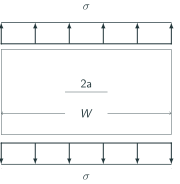
\includegraphics{../images/center-finite.svg}
\caption{center crack, finite width}
\end{figure}
\end{frame}

\begin{frame}{center crack, finite width}
\protect\hypertarget{center-crack-finite-width-1}{}
\[K_I = \sigma \sqrt{\pi a} \sqrt{\sec (\pi a/W)}\] - Accurate within
0.3\% for \(2a/W \le 0.7\) - within 1.0\% for \(2a/W = -.8\)
\[K_I = \sigma \sqrt{\pi a} \left[1.0 - 0.025\left(\frac{2a}{W}\right)^2 + 0.06\left(\frac{2a}{W}\right)^4\right]\sqrt{\sec (\pi a/W)}\]
- Accurate within 0.1\% for all crack lengths.
\end{frame}

\begin{frame}{edge crack, semi-infinite width}
\protect\hypertarget{edge-crack-semi-infinite-width}{}
\[K_I = 1.122 \sigma \sqrt{\pi a}\]
\includegraphics{../images/edge-infinite.svg}
\end{frame}

\begin{frame}{edge crack, finite width}
\protect\hypertarget{edge-crack-finite-width}{}
\begin{figure}
\centering
\includegraphics{../images/edge-finite.svg}
\caption{edge crack, finite width}
\end{figure}
\end{frame}

\begin{frame}{edge crack, finite width}
\protect\hypertarget{edge-crack-finite-width-1}{}
\[\beta = \left[1.122 - 0.231 \frac{a}{W} + 10.55 \left(\frac{a}{W}\right)^2 - 21.71 \left(\frac{a}{W}\right)^3 + 30.82 \left(\frac{a}{W}\right)^4\right]\]

\begin{itemize}
\tightlist
\item
  Within 0.5\% accuracy for \(\frac{a}{W} < 0.6\)
\end{itemize}

\[\beta = \frac{0.752 + 2.02\frac{a}{W} + 0.37\left(1-\sin \frac{\pi a}{2W}\right)^3}{\cos \frac{\pi a}{2W}}\sqrt{\frac{2W}{\pi a} \tan \frac{\pi a}{2W}}\]

\begin{itemize}
\tightlist
\item
  Within 0.5\% accuracy for \(0 < \frac{a}{W} < 1.0\)
\end{itemize}
\end{frame}

\begin{frame}{edge crack, bending moment}
\protect\hypertarget{edge-crack-bending-moment}{}
\begin{figure}
\centering

\includegraphics{../images/bending.svg}
\caption{edge crack under bending}
\end{figure}
\end{frame}

\begin{frame}{edge crack, bending moment}
\protect\hypertarget{edge-crack-bending-moment-1}{}
\begin{itemize}
\tightlist
\item
  The usual form for stress intensity still applies
  \[K_I = \sigma \sqrt{\pi a} \beta\]
\item
  Where \(\sigma = \frac{6M}{tW^2}\)
  \[\beta = 1.122 - 1.40 \left(\frac{a}{W}\right) + 7.33 \left(\frac{a}{W}\right)^2 - 13.08\left(\frac{a}{W}\right)^3 + 14.0 \left(\frac{a}{W}\right)^4\]
\item
  valid within 0.2\% accuracy for \(\frac{a}{W} \le 0.6\)
\end{itemize}
\end{frame}

\begin{frame}{edge crack, bending moment}
\protect\hypertarget{edge-crack-bending-moment-2}{}
\[\beta = \frac{0.923 + 0.199 \left(1-\sin \frac{\pi a}{2W}\right)^4}{\cos \frac{\pi a}{2W}}\sqrt{\frac{2W}{\pi a} \tan \frac{\pi a}{2W}}\]
- valid within 0.5\% for any \(\frac{a}{W}\)
\end{frame}

\begin{frame}{nominal bending stress}
\protect\hypertarget{nominal-bending-stress}{}
\begin{itemize}
\tightlist
\item
  The nominal bending stress is for rectangular cross-sections
\item
  A more general form is given by \(\sigma = \frac{Mc}{I}\)
\item
  Where for a rectangular cross-section, \(c=W/2\) and \(I=tW^3/12\)
  which simplifies as shown previously
\end{itemize}
\end{frame}

\begin{frame}{center crack, finite width, splitting forces}
\protect\hypertarget{center-crack-finite-width-splitting-forces}{}
\begin{figure}
\centering
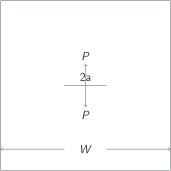
\includegraphics{../images/splitting-force.svg}
\caption{center crack, finite widte, splitting forces}
\end{figure}
\end{frame}

\begin{frame}{center crack, finite width, splitting forces}
\protect\hypertarget{center-crack-finite-width-splitting-forces-1}{}
\begin{itemize}
\tightlist
\item
  With an applied load we use a slightly modified form for the stress
  intensity factor \(K_I = \frac{P}{t \sqrt{\pi a}}\beta\)
\item
  With \(\beta\) in this case given as
  \[\beta = \frac{1 - 0.5\left(\frac{a}{W}\right)+0.975\left(\frac{a}{W}\right)^2 - 0.16\left(\frac{a}{W}\right)^3}{\sqrt{1-\left(\frac{a}{W}\right)}}\]
\end{itemize}
\end{frame}

\begin{frame}{offset crack}
\protect\hypertarget{offset-crack}{}
\begin{figure}
\centering
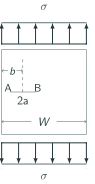
\includegraphics{../images/off-center.svg}
\caption{off-center crack}
\end{figure}
\end{frame}

\begin{frame}{offset crack}
\protect\hypertarget{offset-crack-1}{}
\[K_{IA} = \sigma \sqrt{\pi a} \beta_c \beta_A \text{ and } K_{IB} = \sigma \sqrt{\pi a} \beta_c \beta_B\]

\[ \beta_c = \sqrt{\sec \frac{\pi a}{W}}\]
\end{frame}

\begin{frame}{offset crack}
\protect\hypertarget{offset-crack-2}{}
\[\begin{aligned}
  &\begin{aligned}
  {\beta_A} &= (1-0.025\lambda^2 + 0.6\lambda^4 - \gamma \lambda^{11})\\
  &\qquad \sqrt{\sec \left(\frac{\pi \lambda}{2}\right)\frac{\sin \left(2\lambda - 4\frac{a}{W}\right)}{2\lambda - 4\frac{a}{W}}}
  \end{aligned}\\
  &\begin{aligned}
  {\beta_B} &= (1-0.025\delta^2 + 0.06\delta^4 - \zeta \lambda^{30})\\
  &\qquad \left(1+\frac{\sqrt{\sec\left(\frac{2\pi \lambda + 1.5\pi \delta}{7}\right)-1}}{1+0.21\sin \left( 8 \tan^{-1} \left(\frac{\lambda - \delta}{\lambda + \delta}\right)^{0.9}\right)}\right)
  \end{aligned}
\end{aligned}\] `
\end{frame}

\begin{frame}{offset crack}
\protect\hypertarget{offset-crack-3}{}
\begin{itemize}
\tightlist
\item
  The parameters \(\lambda\), \(\delta\) are given as
\end{itemize}

\[\begin{aligned}
      \lambda &= \frac{a}{b}\\
      \delta &= \frac{a}{W-b}
\end{aligned}\]
\end{frame}

\begin{frame}{offset crack}
\protect\hypertarget{offset-crack-4}{}
\begin{itemize}
\tightlist
\item
  And \(\gamma\) and \(\zeta\) can be looked up on a table
\end{itemize}

\begin{longtable}[]{@{}lll@{}}
\toprule
\(\frac{b}{W}\) & \(\gamma\) & \(\zeta\) \\ \addlinespace
\midrule
\endhead
0.1 & 0.382 & 0.114 \\ \addlinespace
0.25 & 0.136 & 0.286 \\ \addlinespace
0.4 & 0.0 & 0.0 \\ \addlinespace
0.5 & 0.0 & 0.0 \\ \addlinespace
\bottomrule
\end{longtable}
\end{frame}

\begin{frame}{non-uniform stress, infinite width}
\protect\hypertarget{non-uniform-stress-infinite-width}{}
\begin{figure}
\centering
\includegraphics{../images/pressure-function.svg}
\caption{arbitrary pressure function loading along crack}
\end{figure}
\end{frame}

\begin{frame}{non-uniform stress, infinite width}
\protect\hypertarget{non-uniform-stress-infinite-width-1}{}
\begin{itemize}
\tightlist
\item
  Stress intensity will be different at points \(A\) and \$B\$
\end{itemize}

\[\begin{aligned}
    K_{IA} &= \int_{-a}^{a} \frac{p(x)}{\sqrt{\pi a}}\frac{\sqrt{a-x}}{\sqrt{a+x}}dx\\
    K_{IB} &= \int_{-a}^{a} \frac{p(x)}{\sqrt{\pi a}}\frac{\sqrt{a+x}}{\sqrt{a-x}}dx
\end{aligned}\]
\end{frame}

\begin{frame}{cracks around a hole}
\protect\hypertarget{cracks-around-a-hole}{}
\begin{figure}
\centering
\includegraphics{../images/bearing-through.svg}
\caption{a crack around a hole under both remote stress and a local
bearing load}
\end{figure}
\end{frame}

\begin{frame}{cracks around a hole}
\protect\hypertarget{cracks-around-a-hole-1}{}
\begin{itemize}
\tightlist
\item
  For symmetric through cracks under uniform applied stress, we have
\end{itemize}

\[\begin{aligned}
    \beta &= \beta_1 + \beta_2\\
    \beta_1 &= F_{c/R}F_wF_{ww}\\
    \beta_2 &= \frac{\sigma_{br}}{\sigma} F_3 F_w F_{ww}\\
    F_{c/R} &= \frac{3.404 + 3.8172 \frac{c}{R}}{1 + 3.9273\frac{c}{R} - 0.00695 \left(\frac{c}{R}\right)^2 }\\
    F_w &= \sqrt{\sec \frac{\pi R}{W} \sec \frac{\pi (R+c)}{W}}
\end{aligned}\]
\end{frame}

\begin{frame}{cracks around a hole}
\protect\hypertarget{cracks-around-a-hole-2}{}
\[\begin{aligned}
    &\begin{aligned}
    F_{ww} &= 1- \left(\left(1.32 \frac{W}{D} - 0.14\right)^{-(.98+\left(0.1\frac{W}{D}\right)^{0.1})}-0.02\right)\\
    &\qquad \left(\frac{2c}{W-D}\right)^N
    \end{aligned}\\
    F_3 &= 0.098 + 0.3592 e^{-3.5089\frac{c}{R}} + 0.3817 e^{-0.5515 \frac{c}{R}}
\end{aligned}\]
\end{frame}

\begin{frame}{cracks around a hole}
\protect\hypertarget{cracks-around-a-hole-3}{}
\begin{itemize}
\tightlist
\item
  Note that
\end{itemize}

\[\begin{aligned}
  \sigma_{br} &= \frac{P}{Dt}\\
  N &= \frac{W}{D} + 2.5 \qquad \text{when} \qquad \frac{W}{D} < 2\\
  N &= 4.5 \qquad \qquad \text{otherwise}
\end{aligned}\]

\begin{itemize}
\tightlist
\item
  Also \(R\) is the radius, \(R= \frac{D}{2}\)
\end{itemize}
\end{frame}

\begin{frame}{cracks around a hole}
\protect\hypertarget{cracks-around-a-hole-4}{}
\begin{figure}
\centering
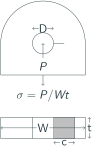
\includegraphics{../images/bearing-single.svg}
\caption{a crack around a hole under both remote stress and a local
bearing load, but there is only a crack on one side}
\end{figure}
\end{frame}

\begin{frame}{cracks around a hole}
\protect\hypertarget{cracks-around-a-hole-5}{}
\[\begin{aligned}
    \beta &= \beta_1 + \beta_2\\
    \beta_1 &= \beta_3 F_w F_{ww}\\
    \beta_2 &= \frac{\sigma_{br}}{\sigma} F_4 F_w F_{ww}\\
    &\begin{aligned}
    \beta_3 &= 0.7071 + 0.7548 \frac{R}{R+c} + 0.3415 \left(\frac{R}{R+C}\right)^2 + \\
    &\qquad 0.6420 \left(\frac{R}{R+c}\right)^3 + 0.9196\left(\frac{R}{R+c}\right)^4
    \end{aligned}\\
    F_4 &= 0.9580 + 0.2561 \frac{c}{R} - 0.00193 \left(\frac{c}{R}\right)^{2.5} - 0.9804 \left(\frac{c}{R}\right)^{0.5}
\end{aligned}\]
\end{frame}

\begin{frame}{cracks around a hole}
\protect\hypertarget{cracks-around-a-hole-6}{}
\[\begin{aligned}
  F_w &= \sqrt{\sec \frac{\pi R}{W} \sec \frac{\pi (R + c/2)}{W-c}}\\
  F_{ww} &= 1 - N^{-\frac{W}{D}} \left(\frac{2c}{W-D}\right)^{\frac{W}{D} + 0.5}\\
  N &= 2.65 - 0.24\left(2.75 - \frac{W}{D}\right)^2\\
  N &\ge 2.275 \qquad \text{(if }N < 2.275\text{, let }N=2.275)
\end{aligned}\]

Also note that \(R\) indicates radius, \(R=\frac{D}{2}\)
\end{frame}

\begin{frame}{group problems}
\protect\hypertarget{group-problems}{}
\begin{enumerate}
\item
  Find \(K_I\) for a center-cracked panel with \(W/2a = 3\) and a
  uniformly applied remote stress, \(\sigma\).
\item
  Find \(K_I\) for an edge-cracked panel with \(W/a = 3\) and a
  uniformly applied remote stress, \(\sigma\).
\item
  Find \(K_I\) for an edge-cracked panel with \(W/a = 3\) and a remote
  bending moment, \(M = tW^2\sigma/6\).
\end{enumerate}
\end{frame}

\begin{frame}{group problems}
\protect\hypertarget{group-problems-1}{}
\begin{enumerate}
\setcounter{enumi}{3}
\item
  Find \(K_I\) for a center-cracked panel with \(W/2a = 3\) and a
  concentrated splitting force, \(P = \sigma a t\).
\item
  What do you think causes the difference (if any) in stress intensity
  between these panels?
\end{enumerate}
\end{frame}

\begin{frame}{example 1}
\protect\hypertarget{example-1}{}
\includegraphics{../images/center-crack.png}
\end{frame}

\begin{frame}{example 1}
\protect\hypertarget{example-1-1}{}
\includegraphics{../images/edge-crack.png}
\end{frame}

\hypertarget{d-crack-shapes}{%
\section{2D crack shapes}\label{d-crack-shapes}}

\begin{frame}{crack depth}
\protect\hypertarget{crack-depth}{}
\begin{itemize}
\tightlist
\item
  The previous stress intensity factors all assume a 2D problem (with a
  1D crack)
\item
  Through the thickness, it is assumed that the crack length is the same
\item
  In many cases this is not an accurate assumption
\item
  We will now consider 2D crack shapes and their effect on the stress
  intensity factor
\end{itemize}
\end{frame}

\begin{frame}{elliptical flaw, infinite solid}
\protect\hypertarget{elliptical-flaw-infinite-solid}{}
\begin{columns}[T]
\begin{column}{0.5\textwidth}
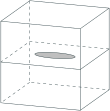
\includegraphics{../images/internal flaw.svg}
\end{column}

\begin{column}{0.5\textwidth}
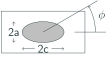
\includegraphics{../images/internal-flaw-in-plane.svg}
\end{column}
\end{columns}
\end{frame}

\begin{frame}{elliptical flaw, infinite solid}
\protect\hypertarget{elliptical-flaw-infinite-solid-1}{}
\begin{itemize}
\tightlist
\item
  For an ellipse the stress intensity factor will vary with the angle,
  \(\phi\)
\end{itemize}

\[\begin{aligned}
  K_I &= \sigma \sqrt{\pi a} \beta\\
  \beta &= \sqrt{\frac{1}{Q}} f_\phi\\
  Q &= 1+ 1.464 \left(\frac{a}{c}\right)^{1.65} \qquad \text{if} a/c \le 1
\end{aligned}\]
\end{frame}

\begin{frame}{elliptical flaw, infinite solid}
\protect\hypertarget{elliptical-flaw-infinite-solid-2}{}
\begin{itemize}
\tightlist
\item
  For an ellipse the stress intensity factor will vary with the angle,
  \(\phi\)
\end{itemize}

\[\begin{aligned}
  Q &= 1+ 1.464 \left(\frac{c}{a}\right)^{1.65} \qquad \text{if} a/c > 1\\
  f_\phi &= \left(\left(\frac{a}{c}\right)^2 \cos^2 \phi + \sin^2 \phi \right)^{1/4}\qquad \text{if} a/c \le 1\\
  f_\phi &= \left(\cos^2 \phi + \left(\frac{c}{a}\right)^2 \sin^2 \phi \right)^{1/4}\qquad \text{if} a/c > 1
\end{aligned}\]
\end{frame}

\begin{frame}{elliptical flaw, finite solid}
\protect\hypertarget{elliptical-flaw-finite-solid}{}
\begin{columns}[T]
\begin{column}{0.5\textwidth}
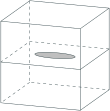
\includegraphics{../images/internal flaw.svg}
\end{column}

\begin{column}{0.5\textwidth}
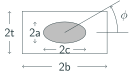
\includegraphics{../images/internal-flaw-finite.svg}
\end{column}
\end{columns}
\end{frame}

\begin{frame}{finite solid}
\protect\hypertarget{finite-solid}{}
\[\begin{aligned}
  \beta &= \sqrt{\frac{1}{Q}} F_e\\
  F_e &= \left(M_1 + M_2 \left(\frac{a}{t}\right)^2 + M_3 \left(\frac{a}{t}\right)^4\right)g f_\phi f_w\\
  f_w &= \sqrt{\sec\left(\frac{\pi c}{2b}\sqrt{\frac{a}{t}}\right)}\\
  g &= 1 - \frac{\left(\frac{a}{t}\right)^4\left(2.6-2\frac{a}{t}\right)^{1/2}}{1+4\frac{a}{c}}\cos \phi
\end{aligned}\]
\end{frame}

\begin{frame}{elliptical flaw, finite solid}
\protect\hypertarget{elliptical-flaw-finite-solid-1}{}
\[\begin{aligned}
    M_2 &= \frac{0.05}{0.11+\left(\frac{a}{c}\right)^{3/2}}\\
    M_3 &= \frac{0.29}{0.23\left(\frac{a}{c}\right)^{3/2}}
\end{aligned}\]
\end{frame}

\begin{frame}{elliptical flaw, finite solid}
\protect\hypertarget{elliptical-flaw-finite-solid-2}{}
\begin{itemize}
\tightlist
\item
  If \(a/c \le 1\) \[\begin{aligned}
  M_1 &= 1\\
  Q &= 1+1.464\left(\frac{a}{c}\right)^{1.65}\\
  f_\phi &= \left(\left(\frac{a}{c}\right)^2 \cos^2 \phi + \sin^2 \phi \right)^{1/4}
  \end{aligned}\]
\end{itemize}
\end{frame}

\begin{frame}{elliptical flaw, finite solid}
\protect\hypertarget{elliptical-flaw-finite-solid-3}{}
\begin{itemize}
\tightlist
\item
  Otherwise (\(a/c > 1\))
\end{itemize}

\[\begin{aligned}
  M_1 &= \left(\frac{c}{a}\right)^{1/2}\\
  Q &= 1+1.464\left(\frac{c}{a}\right)^{1.65}\\
  f_\phi &= \left(\cos^2 \phi + \left(\frac{c}{a}\right)^2 \sin^2 \phi \right)^{1/4}
\end{aligned}\]
\end{frame}

\begin{frame}{semi-elliptical surface flaw, finite body}
\protect\hypertarget{semi-elliptical-surface-flaw-finite-body}{}
\begin{columns}[T]
\begin{column}{0.5\textwidth}
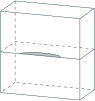
\includegraphics{../images/edge-flaw.svg}
\end{column}

\begin{column}{0.5\textwidth}
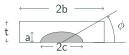
\includegraphics{../images/edge-flaw-plane.svg}
\end{column}
\end{columns}
\end{frame}

\begin{frame}{semi-elliptical surface flaw, finite body}
\protect\hypertarget{semi-elliptical-surface-flaw-finite-body-1}{}
\[\begin{aligned}
  K_I &= \sigma \sqrt{\pi a} \beta\\
  \beta &= \sqrt{\frac{1}{Q}} F_s\\
  F_s &= \left(M_1 + M_2 \left(\frac{a}{t}\right)^2 + M_3 \left(\frac{a}{t}\right)^4\right)g f_\phi f_w\\
  f_w &= \sqrt{\sec\left(\frac{\pi c}{2b}\sqrt{\frac{a}{t}}\right)}
\end{aligned}\]
\end{frame}

\begin{frame}{surface flaw, \(\frac{a}{c} \le 1\)}
\protect\hypertarget{surface-flaw-fracac-le-1}{}
\[\begin{aligned}
  M_1 &= 1.13 - 0.09 \left(\frac{a}{c}\right)\\
  M_2 &= -0.52 + \frac{0.89}{0.2 + \frac{a}{c}}\\
  M_3 &= 0.5 - \frac{1}{0.65 + \frac{a}{c}} + 14 \left(1-\frac{a}{c}\right)^4
\end{aligned}\]
\end{frame}

\begin{frame}{surface flaw, \(\frac{a}{c} \le 1\)}
\protect\hypertarget{surface-flaw-fracac-le-1-1}{}
\[\begin{aligned}
  Q &= 1 + 1.464\left(\frac{a}{c}\right)^{1.65}\\
  f_\phi &= \left(\left(\frac{a}{c}\right)^2 \cos^2 \phi + \sin^2 \phi \right)^{1/4}\\
  g &= 1 + \left(0.1 + 0.35 \left(\frac{a}{t}\right)^2\right)\left(1-\sin \phi\right)^2
\end{aligned}\]
\end{frame}

\begin{frame}{surface flaw, \(\frac{a}{c} > 1\)}
\protect\hypertarget{surface-flaw-fracac-1}{}
\[\begin{aligned}
  M_1 &= \left(\frac{c}{a}\right)^{1/2} \left(1 + 0.04 \frac{c}{a}\right)\\
  M_2 &= 0.2 \left(\frac{c}{a}\right)^4\\
  M_3 &= -0.11 \left(\frac{c}{a}\right)^4
\end{aligned}\]
\end{frame}

\begin{frame}{surface flaw, \(\frac{a}{c} > 1\)}
\protect\hypertarget{surface-flaw-fracac-1-1}{}
\[\begin{aligned}
  Q &= 1 + 1.464\left(\frac{c}{a}\right)^{1.65}\\
  f_\phi &= \left(\cos^2 \phi + \left(\frac{c}{a}\right)^2 \sin^2 \phi \right)^{1/4}\\
  g &= 1 + \left(0.1 + 0.35 \left(\frac{c}{a}\right)\left(\frac{a}{t}\right)^2\right)\left(1-\sin \phi\right)^2
\end{aligned}\]
\end{frame}

\begin{frame}{corner flaw, finite body}
\protect\hypertarget{corner-flaw-finite-body}{}
\begin{columns}[T]
\begin{column}{0.5\textwidth}
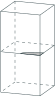
\includegraphics{../images/corner crack.svg}
\end{column}

\begin{column}{0.5\textwidth}
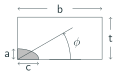
\includegraphics{../images/corner-crack-plane.svg}
\end{column}
\end{columns}
\end{frame}

\begin{frame}{corner flaw, finite body}
\protect\hypertarget{corner-flaw-finite-body-1}{}
\[\begin{aligned}
  K_I &= \sigma \sqrt{\pi a} \beta\\
  \beta &= \sqrt{\frac{1}{Q}} F_c\\
  F_c &= \left(M_1 + M_2 \left(\frac{a}{t}\right)^2 + M_3 \left(\frac{a}{t}\right)^4\right)g_1 g_2 f_\phi f_w\\
  f_w &= 1 - 0.2 \lambda + 9.4 \lambda^2 - 19.4 \lambda^3 + 27.1 \lambda^4\\
  \lambda &= \left(\frac{c}{b}\right)\left(\frac{a}{t}\right)^{1/2}
\end{aligned}\]
\end{frame}

\begin{frame}{corner flaw, finite body, \(\frac{a}{c} \le 1\)}
\protect\hypertarget{corner-flaw-finite-body-fracac-le-1}{}
\[\begin{aligned}
  M_1 &= 1.08 - 0.03 \left(\frac{a}{c}\right)\\
  M_2 &= -0.44 + \frac{1.06}{0.3 + \frac{a}{c}}\\
  M_3 &= -0.5 + 0.25 \frac{a}{c} + 14.8 \left(1-\frac{a}{c}\right)^{1.5}\\
\end{aligned}\]
\end{frame}

\begin{frame}{corner flaw, finite body, \(\frac{a}{c} \le 1\)}
\protect\hypertarget{corner-flaw-finite-body-fracac-le-1-1}{}
\[\begin{aligned}
  Q &= 1 + 1.464\left(\frac{a}{c}\right)^{1.65}\\
  f_\phi &= \left(\left(\frac{a}{c}\right)^2 \cos^2 \phi + \sin^2 \phi \right)^{1/4}\\
  g_1 &= 1 + \left(0.08 + 0.4 \left(\frac{a}{t}\right)^2\right)\left(1-\sin \phi\right)^3\\
  g_2 &= 1 + \left(0.08 + 0.15 \left(\frac{a}{t}\right)^2\right)\left(1-\cos \phi\right)^3
\end{aligned}\]
\end{frame}

\begin{frame}{corner flaw, finite body, \(\frac{a}{c} > 1\)}
\protect\hypertarget{corner-flaw-finite-body-fracac-1}{}
\[\begin{aligned}
  M_1 &= \left(\frac{c}{a}\right)^{1/2} \left(1.08 - 0.03 \frac{c}{a}\right)\\
  M_2 &= 0.375 \left(\frac{c}{a}\right)^4\\
  M_3 &= -0.25 \left(\frac{c}{a}\right)^2
\end{aligned}\]
\end{frame}

\begin{frame}{corner flaw, finite body, \(\frac{a}{c} > 1\)}
\protect\hypertarget{corner-flaw-finite-body-fracac-1-1}{}
\[\begin{aligned}
  Q &= 1 + 1.464\left(\frac{c}{a}\right)^{1.65}\\
  f_\phi &= \left(\cos^2 \phi + \left(\frac{c}{a}\right)^2 \sin^2 \phi \right)^{1/4}\\
  g_1 &= 1 + \left(0.08 + 0.4 \left(\frac{c}{t}\right)^2\right)\left(1-\sin \phi\right)^3\\
  g_2 &= 1 + \left(0.08 + 0.15 \left(\frac{c}{t}\right)^2\right)\left(1-\cos \phi\right)^3
\end{aligned}\]
\end{frame}

\begin{frame}{example 2}
\protect\hypertarget{example-2}{}
:::::::::::::: \{.columns\} ::: \{.column width=``50\%''\}
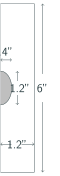
\includegraphics{../images/example-1.svg}

::: ::: \{.column width=``50\%''\}

Find maximum value of \(K_I\) for semi-elliptical surface flaw

\(\sigma = 20 \text{ kpsi}\) (in opening direction)

::: ::::::::::::::
\end{frame}

\begin{frame}{example 2}
\protect\hypertarget{example-2-1}{}
\begin{itemize}
\tightlist
\item
  Here we will use the formula for a semi-elliptical surface flaw
\item
  In the first step we find \(a/c = 0.4/0.6 < 1\), so we use that set of
  formulae
\item
  A worked python notebook of this example can be found
  \href{../examples/Finite\%20Width.html}{here}
\end{itemize}
\end{frame}

\hypertarget{d-cracks-at-a-hole}{%
\section{2D cracks at a hole}\label{d-cracks-at-a-hole}}

\begin{frame}{when to consider 2D crack shape}
\protect\hypertarget{when-to-consider-2d-crack-shape}{}
\begin{itemize}
\tightlist
\item
  When do we need to worry about 2D crack shape?
\item
  The important factor is ratio of crack length to thickness
\item
  When crack length is less than 5 times thickness, 2D shape effects are
  not negligible
\end{itemize}
\end{frame}

\begin{frame}{cracks around a hole}
\protect\hypertarget{cracks-around-a-hole-7}{}
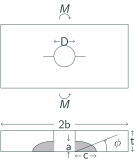
\includegraphics{../images/bearing-symmetric-corner.svg}
\end{frame}

\begin{frame}{remote stress}
\protect\hypertarget{remote-stress}{}
\[\begin{aligned}
  K_{I} &= \sigma \sqrt{\pi a} \beta\\
  \beta &= \sqrt{\frac{1}{Q}} F_{ch}\\
  F_{ch} &= \left(M_1 + M_2 \left(\frac{a}{t}\right)^2 + M_3 \left(\frac{a}{t}\right)^4\right)g_1 g_2 g_3 g_4 f_\phi f_w\\
  f_w &= \sqrt{\sec \left(\frac{\pi r}{2b}\right)\sec \left(\frac{\pi (2r + nc)}{4(b-c) + 2nc} \sqrt{\frac{a}{t}}\right)}
\end{aligned}\]
\end{frame}

\begin{frame}{remote stress}
\protect\hypertarget{remote-stress-1}{}
\[\begin{aligned}
  g_2 &= \frac{1+0.358\lambda+1.425\lambda^2 - 1.578\lambda^3+2.156\lambda^4}{1+0.13\lambda^2}\\
  \lambda &= \frac{1}{1+(c/r)\cos \left(0.85 \phi \right)}
\end{aligned}\] Where \(n =\) number of cracks (1 or 2)
\end{frame}

\begin{frame}{remote stress when \(a/c \le 1\)}
\protect\hypertarget{remote-stress-when-ac-le-1}{}
\[\begin{aligned}
  M_1 &= 1.13 - 0.09 \left(a/c\right)\\
  M_2 &= -0.54 + \frac{0.89}{0.2 + a/c}\\
  M_3 &= 0.5 - \frac{1}{0.65 + a/c}+ 14 \left(1-a/c\right)^{24}\\
  Q &= 1+1.464\left(a/c\right)^{1.65}
\end{aligned}\]
\end{frame}

\begin{frame}{remote stress when \(a/c \le 1\)}
\protect\hypertarget{remote-stress-when-ac-le-1-1}{}
\[\begin{aligned}
  g_1 &= 1 + \left(0.1+0.35 \left(a/t\right)^2\right)(1-\sin \phi)^2\\
  g_3 &= (1+0.04 (a/c))\left(1+0.1(1-\cos \phi)^2\right)\left(0.85+0.15(a/t)^{1/4}\right)\\
  g_4 &= 1 - 0.7(1-a/t)(a/c-0.2)(1-a/c)\\
  f_\phi &= \left(\left(a/c\right)^2 \cos^2 \phi + \sin^2 \phi \right)^{1/4}
\end{aligned}\]
\end{frame}

\begin{frame}{remote stress when \(a/c > 1\)}
\protect\hypertarget{remote-stress-when-ac-1}{}
\[\begin{aligned}
  M_1 &= \sqrt{c/a}(1+0.04 (c/a))\\
  M_2 &= 0.2(c/a)^4\\
  M_3 &= -0.11(c/a)^4\\
  Q &= 1+1.464\left(\frac{c}{a}\right)^{1.65}
\end{aligned}\]
\end{frame}

\begin{frame}{remote stress when \(a/c > 1\)}
\protect\hypertarget{remote-stress-when-ac-1-1}{}
\[\begin{aligned}
  g_1 &= 1 + \left(0.1+0.35 (c/a)\left(a/t\right)^2\right)(1-\sin \phi)^2\\
  g_3 &= (1.13-0.09 (c/a))\left(1+0.1(1-\cos \phi)^2\right)\left(0.85+0.15(a/t)^{1/4}\right)\\
  g_4 &= 1 \\
  f_\phi &= \left(\cos^2 \phi + \left(\frac{c}{a}\right)^2 \sin^2 \phi \right)^{1/4}
\end{aligned}\]
\end{frame}

\begin{frame}{remote stress}
\protect\hypertarget{remote-stress-2}{}
\begin{itemize}
\tightlist
\item
  The same formulas apply for both symmetric cracks (\(n=2\)) and a
  single crack (\(n=1\)) with one additional correction factor applied
  to the single crack case
  \[K_{I,single} = \sqrt{\frac{4/\pi + ac/2tr}{4/\pi + ac/tr}}K_{I,symmetric}\]
\end{itemize}
\end{frame}

\begin{frame}{surface cracks around a hole}
\protect\hypertarget{surface-cracks-around-a-hole}{}
\includegraphics{../images/bearing-surface.svg}
\end{frame}

\begin{frame}{remote stress}
\protect\hypertarget{remote-stress-3}{}
\[\begin{aligned}
  K_{I} &= \sigma \sqrt{\pi a} \beta\\
  \beta &= \sqrt{\frac{1}{Q}} F_{sh}\\
  F_{sh} &= \left(M_1 + M_2 \left(\frac{a}{t}\right)^2 + M_3 \left(\frac{a}{t}\right)^4\right)g_1 g_2 g_3 f_\phi f_w\\
  f_w &= \sqrt{\sec \left(\frac{\pi r}{2b}\right)\sec \left(\frac{\pi (2r + nc)}{4(b-c) + 2nc} \sqrt{\frac{a}{t}}\right)}
\end{aligned}\]
\end{frame}

\begin{frame}{remote stress}
\protect\hypertarget{remote-stress-4}{}
\[\begin{aligned}
  M_2 &= \frac{0.05}{0.11 + (a/c)^{3/2}}\\
  M_3 &= \frac{0.29}{0.23 + (a/c)^{3/2}}
\end{aligned}\] Where \(n =\) number of cracks (1 or 2)
\end{frame}

\begin{frame}{remote stress}
\protect\hypertarget{remote-stress-5}{}
\[\begin{aligned}
  g_1 &= 1- \frac{(a/t)^4(2.6-2a/t)^{1/2}}{1+4a/c}\cos \phi\\
  g_2 &= \frac{1+0.358\lambda+1.425\lambda^2 - 1.578\lambda^3+2.156\lambda^4}{1+0.08\lambda^2}\\
  \lambda &= \frac{1}{1+(c/r)\cos \left(0.9 \phi \right)}\\
  g_3 &= 1+0.1(1-\cos \phi)^2 (1-a/t)^{10}
\end{aligned}\]
\end{frame}

\begin{frame}{remote stress \(a/c \le 1\)}
\protect\hypertarget{remote-stress-ac-le-1}{}
\[\begin{aligned}
  Q &= 1 + 1.464(a/c)^{1.65}\\
  M_1 &= 1\\
  f_\phi &= \left(\left(\frac{a}{c}\right)^2 \cos^2 \phi + \sin^2 \phi \right)^{1/4}
\end{aligned}\]
\end{frame}

\begin{frame}{remote stress \(a/c > 1\)}
\protect\hypertarget{remote-stress-ac-1}{}
\[\begin{aligned}
  Q &= 1 + 1.464(c/a)^{1.65}\\
  M_1 &= \sqrt{c/a}\\
  f_\phi &= \left(\cos^2 \phi + \left(\frac{c}{a}\right)^2 \sin^2 \phi \right)^{1/4}
\end{aligned}\]
\end{frame}

\begin{frame}{single-crack correction}
\protect\hypertarget{single-crack-correction}{}
\begin{itemize}
\tightlist
\item
  When the surface crack is only on one side of the hole, we use the
  same correction as for corner cracks
  \[K_{I,single} = \sqrt{\frac{4/\pi + ac/2tr}{4/\pi + ac/tr}}K_{I,symmetric}\]
\end{itemize}
\end{frame}

\begin{frame}{edge crack on a lug}
\protect\hypertarget{edge-crack-on-a-lug}{}
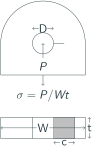
\includegraphics{../images/bearing-single.svg}
\end{frame}

\begin{frame}{edge crack on a lug}
\protect\hypertarget{edge-crack-on-a-lug-1}{}
\[\begin{aligned}
  K_I &= \sigma_{br} \sqrt{\pi c} \beta\\
  \sigma_{br} &= P/Dt\\
  \beta &= \left(\frac{G_0 D}{2W} + G_1\right)G_w G_L G_2\\
  z &= \left(1+\frac{2C}{D}\right)^{-1}\\
  G_0 &= 0.7071 + 0.7548z + 0.3415z^2 + 0.642z^3 + 0.9196z^4\\
  G_1 &= 0.078z + 0.7588z^2 - 0.4293z^3 + 0.0644z^4 + 0.651z^5\\
  G_L &= \left(\sec \left(\frac{\pi D}{2W}\right)\right)^{1/2}
\end{aligned}\]
\end{frame}

\begin{frame}{edge crack on a lug}
\protect\hypertarget{edge-crack-on-a-lug-2}{}
\[\begin{aligned}
  \lambda &= \frac{\pi}{2} \left(\frac{D+c}{W-c}\right)\\
  G_w &= \left(\sec \lambda \right)^{1/2}\\
  b &= \frac{W-D}{2}\\
  A_1 &= 0.688 + 0.772 \frac{D}{W} + 0.613 \left(\frac{D}{W}\right)^2\\
  A_2 &= 4.948 - 17.318 \frac{D}{W} + 16.785 \left(\frac{D}{W}\right)^2
\end{aligned}\]
\end{frame}

\begin{frame}{edge crack on a lug}
\protect\hypertarget{edge-crack-on-a-lug-3}{}
\[\begin{aligned}
    A_3 &= -14.297 + 62.994 \frac{D}{W} - 69.818 \left(\frac{D}{W}\right)^2\\
    A_4 &= 12.35 - 58.644 \frac{D}{W} + 66.387 \left(\frac{D}{W}\right)^2\\
    G_2 &= A_1 + A_2 \frac{c}{b} + A_3 \left(\frac{c}{b}\right)^2 + A_4 \left(\frac{c}{b}\right)^3
\end{aligned}\]
\end{frame}

\begin{frame}{corner crack on a lug}
\protect\hypertarget{corner-crack-on-a-lug}{}
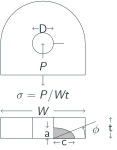
\includegraphics{../images/bearing-single-corner.svg}
\end{frame}

\begin{frame}{corner crack on a lug}
\protect\hypertarget{corner-crack-on-a-lug-1}{}
\[\begin{aligned}
  \beta &= \left(\frac{G_0 D}{2W} + G_1\right)G_w\\
  z &= \left(1 + 2\frac{c}{D} \cos (0.85 \phi)\right)^{-1}\\
  f_0(z) &= 0.7071 + 0.7548z + 0.3415z^2 + 0.642z^3 + 0.9196z^4\\
  f_1(z) &= 0.078z + 0.7588z^2 - 0.4293z^3 + 0.0644z^4 + 0.651z^5\\
  G_0 &= \frac{f_0(z)}{d_0}\\
  d_0 &= 1 + 0.13z^2
\end{aligned}\]
\end{frame}

\begin{frame}{corner crack on a lug}
\protect\hypertarget{corner-crack-on-a-lug-2}{}
\[\begin{aligned}
  g_p &= \left(\frac{W+D}{W-D}\right)^{1/2}\\
  G_1 &= f_1(z) \left(\frac{g_p}{d_0}\right)\\
  G_w &= M_0 g_1 g_3 g_4 f_\phi f_w f_x\\
  v &= \frac{a}{t}
\end{aligned}\]
\end{frame}

\begin{frame}{corner crack on a lug}
\protect\hypertarget{corner-crack-on-a-lug-3}{}
\[\begin{aligned}
  \lambda &= \frac{\pi}{2} \sqrt{v} \left(\frac{D+c}{W-c}\right)\\
  f_w &= \left(\sec \lambda \sec \frac{\pi D}{2W}\right)^{1/2}\\
  x &= \frac{a}{c}
\end{aligned}\]
\end{frame}

\begin{frame}{corner crack on a lug \(a/c \le 1\)}
\protect\hypertarget{corner-crack-on-a-lug-ac-le-1}{}
\[
\begin{aligned}
  f_\phi &= \left(\left(\frac{a}{c}\cos \phi\right)^2 + \sin^2 \phi \right)^{1/4}\\
  f_x &= \left(1+1.464 \left(\frac{a}{c}\right)^{1.65}\right)^{-1/2}\\
  &\begin{aligned}
    M_0 &= (1.13 - 0.09x) + \left(-0.54 + \frac{0.89}{0.2 + x}\right)v^2 {    \colorbox{red}{+}} \\
    &\qquad \left(0.5 - \frac{1}{.65-x} + 14(1-x^{24})\right)v^4
  \end{aligned}
\end{aligned}\]
\end{frame}

\begin{frame}{corner crack on a lug \(a/c \le 1\)}
\protect\hypertarget{corner-crack-on-a-lug-ac-le-1-1}{}
\[\begin{aligned}
  g_1 &= 1 + \left(0.1 + 0.35 v^2\right)\left(1-\sin \phi\right)^2\\
  g_3 &= \left(1+0.04x\right)\left(1 + 0.1 \left(1-\cos \phi \right)^2\right)\left(0.85 + 0.15v ^{1/4}\right)\\
  g_4 &= 1 - 0.7 \left(1-v\right)\left(x - 0.2\right)\left(1-x\right)
\end{aligned}\]
\end{frame}

\begin{frame}{corner crack on a lug \(a/c > 1\)}
\protect\hypertarget{corner-crack-on-a-lug-ac-1}{}
\[\begin{aligned}
  f_\phi &= \left(\left(\frac{ac}{c} \sin \phi \right)^2 + \cos^2 \phi \right)^{1/4}\\
  f_x &= \left(1 + 1.464 \left(\frac{c}{a}\right)^{1.65}\right)^{-1/2}\\
  M_0 &= x^{-1/2} + 0.04 x^{-3/2} + 0.2 x^{-4} v^2  - 0.11 x^{-4}v^4
\end{aligned}\]
\end{frame}

\begin{frame}{corner crack on a lug \(a/c > 1\)}
\protect\hypertarget{corner-crack-on-a-lug-ac-1-1}{}
\[\begin{aligned}
  g_1 &= 1 + \left(0.1 + \frac{0.35}{x}v^2\right)\left(1-\sin \phi \right)^2\\
  g_3 &= \left(1.13 + \frac{0.09}{x}\right)\left(1+0.1(1-\cos \phi)^2\right)\left(0.85 + 0.15v^{1/4}\right)\\
  g_4 &= 1
\end{aligned}\]
\end{frame}

\begin{frame}{symmetric corner cracks under bending}
\protect\hypertarget{symmetric-corner-cracks-under-bending}{}
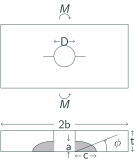
\includegraphics{../images/bearing-symmetric-corner.svg}
\end{frame}

\begin{frame}{corner cracks under bending}
\protect\hypertarget{corner-cracks-under-bending}{}
\[\begin{aligned}
  \sigma_b &= \frac{Mt}{2 I}\\
  I &= \frac{bt^3}{6}\\
  \beta &= H_{ch} \left(\frac{a}{cQ}\right)^{1/2} F_{ch}
\end{aligned}\]
\end{frame}

\begin{frame}{corner cracks under bending}
\protect\hypertarget{corner-cracks-under-bending-1}{}
\[\begin{aligned}
  H_{ch} &= H_1 + (H_2 - H_1) \sin ^p \phi\\
  H_1 &= 1 + G_{11} (a/t) + G_{12} (a/t)^2 + G_{13} (a/t)^3\\
  H_2 &= 1 + G_21 (a/t) + G_{22}(a/t)^2 + G_{23}(a/t)^3
\end{aligned}\]
\end{frame}

\begin{frame}{corner cracks under bending}
\protect\hypertarget{corner-cracks-under-bending-2}{}
\[\begin{aligned}
  F_{ch} &= \left(M_1 + M_2(a/t)^2 + M_3(a/t)^4\right)g_1 g_2 g_3 g_4 f_\phi f_w\\
  \lambda &= \frac{1}{1 + (c/r) \cos (0.85 \phi)}\\
  g_2 &= \frac{1 + .358 \lambda + 1.425 \lambda^2 - 1.578 \lambda^3 + 2.156 \lambda^4}{1 + 0.13\lambda^2}
\end{aligned}\]
\end{frame}

\begin{frame}{corner cracks under bending \(a/c \le 1\)}
\protect\hypertarget{corner-cracks-under-bending-ac-le-1}{}
\[\begin{aligned}
  M_1 &= 1.13 - 0.09 (a/c)\\
  M_2 &= -0.54 + \frac{0.89}{0.2 + a/c}\\
  M_3 &= 0.5 - \frac{1}{0.65+a/c} + 14(1-a/c)^4\\
  Q &= 1 + 1.464(a/c)1.65
\end{aligned}\]
\end{frame}

\begin{frame}{corner cracks under bending \(a/c \le 1\)}
\protect\hypertarget{corner-cracks-under-bending-ac-le-1-1}{}
\[\begin{aligned}
  g_1 &= 1 + \left(0.1 + (a/t) v^2\right)\left(1-\sin \phi\right)^2\\
  g_3 &= \left(1+0.04 (a/c) \right)\left(1 + 0.1 \left(1-\cos \phi \right)^2\right)\left(0.85 + 0.15(a/t) ^{1/4}\right)\\
  g_4 &= 1 - 0.7 \left(1-a/t\right)\left(a/c - 0.2\right)\left(1-a/c\right)
\end{aligned}\]
\end{frame}

\begin{frame}{corner cracks under bending}
\protect\hypertarget{corner-cracks-under-bending-3}{}
\[\begin{aligned}
  f_\phi &= \left(\left(\frac{a}{c}\cos \phi\right)^2 + \sin^2 \phi \right)^{1/4}\\
  G_{11} &= -0.43 - 0.74 a/c - 0.84 (a/c)^2\\
  G_{12} &= 1.25 - 1.19 a/c + 4.39 (a/c)^2\\
  G_{13} &= -1.94 + 4.22 a/c - 5.51 (a/c)^2
\end{aligned}\]
\end{frame}

\begin{frame}{corner cracks under bending}
\protect\hypertarget{corner-cracks-under-bending-4}{}
\[\begin{aligned}
  G_{21} &= -1.5 - 0.04 a/c - 1.73 (a/c)^2\\
  G_{22} &= 1.71 - 3.17 a/c + 6.84 (a/c)^2\\
  G_{23} &= -1.28 + 2.71 a/c - 5.22 (a/c)^2\\
  p &= 0.1 + 1.3 a/t + 1.1 a/c - 0.7 (a/c) (a/t)
\end{aligned}\]
\end{frame}

\begin{frame}{corner cracks under bending \(a/c > 1\)}
\protect\hypertarget{corner-cracks-under-bending-ac-1}{}
\[\begin{aligned}
  M_1 &= (c/a)^{1/2}(1+0.04 c/a)\\
  M_2 &= 0.2 (c/a)^4\\
  M_3 &= -0.11 (c/a)^4\\
  Q &= 1+ 1.464(c/a)^{1.65}\\
  g_1 &= 1 + \left(0.1 0.35(c/a)(a/t)^2\right)\left(1-\sin \phi\right)^2\\
  g_3 &= \left(1.13 - 0.09(c/a)\right)\left(1+ 0.1(1-\cos \phi)^2\right)\left(0.85 + 0.15(a/t)^{1/4}\right)\\
  g_4 &= 1
\end{aligned}\]
\end{frame}

\begin{frame}{corner cracks under bending}
\protect\hypertarget{corner-cracks-under-bending-5}{}
\[\begin{aligned}
  f_\phi &= \left(\left(\cos^2 \phi + \frac{c}{a}\sin \phi\right)^2  \right)^{1/4}\\
  G_{11} &= -2.07 + 0.06 c/a\\
  G_{12} &= 4.35 + 0.16 c/a\\
  G_{13} &= -2.93 - 0.3c/a
\end{aligned}\]
\end{frame}

\begin{frame}{corner cracks under bending}
\protect\hypertarget{corner-cracks-under-bending-6}{}
\[\begin{aligned}
  G_{21} &= -3.64 + 0.37c/a\\
  G_{22} &= 5.87 - 0.49c/a\\
  G_{23} &= -4.32 + 0.53c/a\\
  p &= 0.2 + c/a + 0.6a/t
\end{aligned}\]
\end{frame}

\begin{frame}{example 3}
\protect\hypertarget{example-3}{}
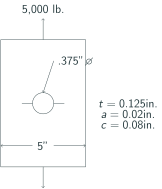
\includegraphics{../images/example 2.svg}
\end{frame}

\begin{frame}{example}
\protect\hypertarget{example}{}
\begin{itemize}
\tightlist
\item
  Case 1 - symmetric through cracks
\item
  Case 2 - single through crack
\item
  Case 3 - symmetric corner cracks
\item
  Case 4 - single corner crack
\item
  Case 5 - symmetric surface cracks
\item
  Case 6 - single surface crack
\item
  Viewable \href{../examples/Cracks\%20Around\%20a\%20Hole.html}{here}
\end{itemize}
\end{frame}

\end{document}
